\documentclass[10pt,twocolumn]{article}
\usepackage[margin=0.70in]{geometry}
\usepackage{amsmath,amssymb,amsthm}
\usepackage{booktabs}
\usepackage{graphicx}
\usepackage{xcolor}
\usepackage{hyperref}
\usepackage{enumitem}
\usepackage{listings}

\hypersetup{
  colorlinks=true,
  linkcolor=blue!60!black,
  citecolor=blue!60!black,
  urlcolor=blue!60!black
}

\lstset{
  basicstyle=\ttfamily\scriptsize,
  columns=fullflexible,
  frame=single,
  breaklines=true,
  rulecolor=\color{black!25},
  backgroundcolor=\color{black!2}
}

\newtheorem{theorem}{Theorem}[section]
\newtheorem{lemma}[theorem]{Lemma}
\newtheorem{proposition}[theorem]{Proposition}
\newtheorem{corollary}[theorem]{Corollary}
\theoremstyle{definition}
\newtheorem{definition}[theorem]{Definition}
\newtheorem{remark}[theorem]{Remark}

\title{\textbf{Machine-Checked Robotics and Control Verification in Lean~4:\\
The \texttt{Robotics} Proof Library, \texttt{ctrl.robotics} Dual-Mode Runtime \& C99/ST Codegen,\\
and Closed-Loop MuJoCo Physics Benchmarks}}

\author{Mike Helsel\\
\small \texttt{ctrl} Formal Robotics \& Control Laboratory}
\date{October 19, 2026}

\begin{document}
\maketitle

\begin{abstract}
Modern robotic locomotion, manipulation, state estimation, and visual servoing stacks rely on implicit analytical assumptions across trajectory generation, real-time clock synchronization, contact wrench allocation, projective camera geometry, and linear-quadratic estimation and control. We present an end-to-end formally verified robotics software and proof ecosystem coupling a 63-module, 21,937-line Lean~4 library (\texttt{lean/Robotics}, built on Mathlib with zero \texttt{sorry} and only the standard foundational axioms \texttt{propext}, \texttt{Classical.choice}, and \texttt{Quot.sound}) with a dual-mode Python/NumPy/$\mathbb{Q}$ runtime library (\texttt{ctrl.robotics}), a deterministic C99 and IEC~61131-3 Structured Text code generator, and a closed-loop MuJoCo~3.16 physics benchmark suite. Our contributions span six pillars:
(1)~\textbf{Strict Energy Pareto Dominance over Minimum-Jerk}: Using the Fundamental Theorem of Calculus on explicit degree-13/11/9 polynomial antiderivatives, we prove that the classical Flash--Hogan quintic minimum-jerk trajectory ($\eta = 0$) is \emph{strictly Pareto-dominated} across the entire septic family interval $\eta \in [-11, 0)$ for both electrical $I^2R$ Joule heating ($\int_0^T \ddot{q}(t)^2\,dt$, reduced by exactly $11/60 \approx 18.33\%$ at $\eta = -11$) and mechanical viscous dissipation ($\int_0^T \dot{q}(t)^2\,dt$, reduced by exactly $421/3900 \approx 10.79\%$ at $\eta = -11$), while conservative inertial cross-power $\int_0^T \dot{q}\ddot{q}\,dt = 0$ vanishes identically on every rest-to-rest motion;
(2)~\textbf{World-Frame Transport, Redundant Nullspace Allocation, and Clock-Slew Hazards}: We prove Euler--centripetal orthogonality ($\boldsymbol{\alpha}\times\mathbf{p} \perp \boldsymbol{\omega}\times(\boldsymbol{\omega}\times\mathbf{p})$), exact Pythagorean $L^2$ optimality of Moore--Penrose minimal-intervention inverse kinematics, third-order time-warp chain rules establishing that piecewise-linear clock slewing destroys $C^1$ spline differentiability, and arrival-curve event-queue bounds;
(3)~\textbf{3D Four-Contact Lorentz-Cone ZMP \& Continuous-Time CBF Invariance}: We formalize a 3D rectangular four-contact bilinear Zero Moment Point (ZMP) normal load and proportional shear allocator that realizes $(m a_x, m a_y, 0)$ with zero 3D angular-momentum drift ($\dot{\mathbf{L}} = \mathbf{0}$ across roll, pitch, and yaw), preserves each foot's second-order Lorentz friction cone $\mathcal{K}(\mu)$, and guarantees continuous-time ODE forward invariance;
(4)~\textbf{6-DOF $SE(3)$ Visual Servoing Depth Positivity \& Homography Decomposition}: We prove that rotational angular velocity $\boldsymbol{\omega}(t)$ cancels identically in the 6-DOF plane-depth Lie derivative $\frac{d}{dt}(\mathbf{n}_c\cdot\mathbf{X}_c) = -\mathbf{n}_c\cdot\mathbf{v}$, prove Faugeras--Lustman 8-to-2 chirality elimination, and establish from first principles that $\mathbf{w} = \mathbf{n}\times\mathbf{v}$ is an exact unit singular vector ($\sigma_2 = 1$) of $H = I + \mathbf{v}\mathbf{n}^\top$ satisfying $(\sigma_1^2 - 1)(1 - \sigma_3^2) = \|\mathbf{n}\times\mathbf{v}\|^2 \ge 0$;
(5)~\textbf{Verified Estimation, LQR/DARE, MPC, and Real-Time Scheduling}: We unify 45 modules in \texttt{ControlsLean} and \texttt{RoboLean} covering DARE Bellman completion of squares, Bucy--Joseph Kalman MMSE trace optimality, Kalata's $\alpha$-$\beta$ tracking relation, Luenberger separation, constrained MPC Lyapunov descent, and Joseph--Pandya / Liu--Layland / EDF real-time schedulability; and
(6)~\textbf{Executable Verification Pipeline (\texttt{ctrl robotics-check})}: Every public Python function is bound via \texttt{@lean\_theorem} to its Lean~4 proof, verified against exact rational ($\mathbb{Q}$) certificates, compiled to zero-heap C99 (\texttt{clang -O3}, $< 4.5\times 10^{-16}$ parity error) and IEC~61131-3 ST, and validated in closed-loop MuJoCo~3.16 physics rollouts.
\end{abstract}

\section{Introduction and System Architecture}

Safety-critical robotic systems combine continuous-time physical mechanics with discrete-time digital execution, optimization-based safety filters, state estimators, and multi-view geometric perception. Subtle analytical bugs frequently arise at the boundaries between these layers:
\begin{itemize}[leftmargin=1.4em,itemsep=2pt]
  \item \textbf{Trajectory smoothness vs.\ actuator thermal limits}: Minimum-jerk quintic polynomials~\cite{FlashHogan1985} are universally deployed as default point-to-point motion primitives under the assumption that smoothness minimizes actuator effort. Yet in direct-drive and quasi-direct-drive actuators, thermal saturation is governed by winding $I^2R$ Joule loss ($\propto \int \tau^2\,dt$) and joint viscous dissipation ($\propto \int \dot{q}^2\,dt$).
  \item \textbf{Networked clock synchronization}: Distributed EtherCAT and ROS~2 motion controllers synchronize local servo clocks via PTP/NTP rate slewing ($\tau(t) = t_k + \alpha (t - t_k)$). Engineers routinely assume that composing a $C^2$ spline with a continuous clock warp preserves $C^2$ trajectory smoothness.
  \item \textbf{3D contact wrench realizability}: Planar inverted-pendulum braking limits ($a_{\max} = g\min(\mu, W/h_G)$) neglect three-dimensional roll/pitch/yaw moment coupling and four-contact second-order Lorentz friction-cone feasibility.
  \item \textbf{Visual servoing chirality and depth}: Homography-based visual servoing (HBVS)~\cite{MalisChaumette2000} and planar homography decomposition~\cite{FaugerasLustman1988} rely on algebraic singular-value separation ($\sigma_1 \ge \sigma_2 = 1 \ge \sigma_3$), two-view cheirality~\cite{HartleyZisserman2004}, and rotational invariance of scene depth under arbitrary 6-DOF camera angular velocity $\boldsymbol{\omega}(t) \in \mathbb{R}^3$.
\end{itemize}

\begin{table*}[t]
\centering
\caption{\textbf{Architecture of the Unified \texttt{lean/Robotics} Proof Library and \texttt{ctrl.robotics} Runtime Stack.} All 63 Lean~4 modules (21,937 LOC, 1,955 declarations) compile under a single \texttt{lake build Robotics} target with zero \texttt{sorry}, zero \texttt{native\_decide}, and standard axioms only.}
\label{tab:architecture}
\vspace{2pt}
\scriptsize
\setlength{\tabcolsep}{4pt}
\begin{tabular}{@{}llrrll@{}}
\toprule
\textbf{Subsystem} & \textbf{Lean~4 Namespace} & \textbf{Files} & \textbf{LOC} & \textbf{Python Module} & \textbf{Key Verified Kernels \& Theorems} \\
\midrule
Trajectory \& Energy & \texttt{Research.RobotEnergy*} & 1 & 386 & \texttt{trajectories.py} & Septic $q_\eta, v_\eta, a_\eta, j_\eta$, $I_v, I_a, I_j$, Pareto $\eta \in [-11, 0)$ \\
Transport, IK \& Clock & \texttt{Research.WorldFrame*} & 1 & 390 & \texttt{kinematics\_ik.py} & $\boldsymbol{\alpha}\times\mathbf{p} \perp \boldsymbol{\omega}\times(\boldsymbol{\omega}\times\mathbf{p})$, Pythagorean IK, clock-slew jump \\
3D Contact \& CBF & \texttt{Research.Lorentz*}, \texttt{Centroidal*} & 4 & 1,417 & \texttt{contact\_cbf.py} & 4-contact bilinear ZMP ($\dot{\mathbf{L}}=\mathbf{0}$), Lorentz $\mathcal{K}(\mu)$, ODE CBF \\
6-DOF Vision \& $SE(3)$ & \texttt{Research.Homography*}, \texttt{Visual*} & 2 & 1,015 & \texttt{vision\_se3.py} & $G(\mathbf{n}\times\mathbf{v})=\mathbf{n}\times\mathbf{v}$, 8$\to$2 chirality, $SE(3)$ depth ODE \\
Controls, LQR \& MPC & \texttt{ControlsLean.Controls.*} & 14 & 4,380 & \texttt{estimation\_lqr.py} & DARE completion of squares, Luenberger separation, MPC CLF \\
Kalman \& Estimation & \texttt{ControlsLean.Estimation.*}, \texttt{Vision.*} & 12 & 4,190 & \texttt{estimation\_lqr.py} & Bucy--Joseph MMSE trace, Kalata $\alpha$-$\beta$ tracker, triangulation \\
Kinematics \& Real-Time & \texttt{RoboLean.*} & 29 & 10,159 & \texttt{kinematics\_ik.py} & $SE(2) \subset E(2)$ clopen, 2-link annulus, RTA, Liu--Layland, EDF \\
\midrule
\textbf{Total / Unified} & \textbf{\texttt{Robotics} Lake Target (\texttt{v4.33.1})} & \textbf{63} & \textbf{21,937} & \textbf{28 Bound Fns} & \textbf{124 Bound Theorems · C99 / ST · MuJoCo~3.16} \\
\bottomrule
\end{tabular}
\end{table*}

To eliminate the gap between paper proofs, theorem-prover scripts, and deployed control code, we built a four-layer verification architecture inside \texttt{ctrl} (summarized in Table~\ref{tab:architecture}):
\begin{enumerate}[leftmargin=1.4em,itemsep=1pt]
  \item \textbf{Unified Lean~4 Proof Library (\texttt{lean/Robotics})}: Consolidates 8 modules in \texttt{Research/}, 26 modules in \texttt{ControlsLean/}, and 29 modules in \texttt{RoboLean/} (63 files, 21,937 lines of Lean~4, 1,955 declarations) under a single \texttt{lake build Robotics} target on Lean \texttt{v4.33.1}.
  \item \textbf{Dual-Mode Python Runtime (\texttt{src/ctrl/robotics/})}: Implements every verified algorithm with polymorphic support for both fast \texttt{float64}/\texttt{NumPy} execution and exact rational \texttt{fractions.Fraction} ($\mathbb{Q}$) arithmetic for zero-rounding certificate generation.
  \item \textbf{Automated Spec-Manifest Audit (\texttt{@lean\_theorem})}: Every public Python function is decorated with \texttt{@lean\_theorem(module, theorems, ...)} in \texttt{registry.py}. Running \texttt{ctrl robotics-check} parses all referenced \texttt{.lean} files, strips comments/strings, verifies that every bound theorem declaration exists, and confirms zero occurrences of \texttt{sorry}, \texttt{admit}, or \texttt{native\_decide}.
  \item \textbf{Deterministic C99 / IEC~61131-3 Codegen \& MuJoCo~3.16 Physics Rollouts}: \texttt{codegen.py} emits dependency-free ANSI C99 (\texttt{ctrl\_robotics\_kernels.h/.c}) and IEC~61131-3 Structured Text (\texttt{.st}) PLC function blocks with embedded Lean~4 theorem provenance headers, compiles the C99 code with \texttt{clang -std=c99 -O3 -Werror}, and verifies bit-level parity ($< 4.44 \times 10^{-16}$) via \texttt{ctypes}, while \texttt{mujoco\_benchmarks.py} validates the controllers in closed-loop MuJoCo~3.16 physics simulations.
\end{enumerate}

\begin{figure*}[t]
\centering
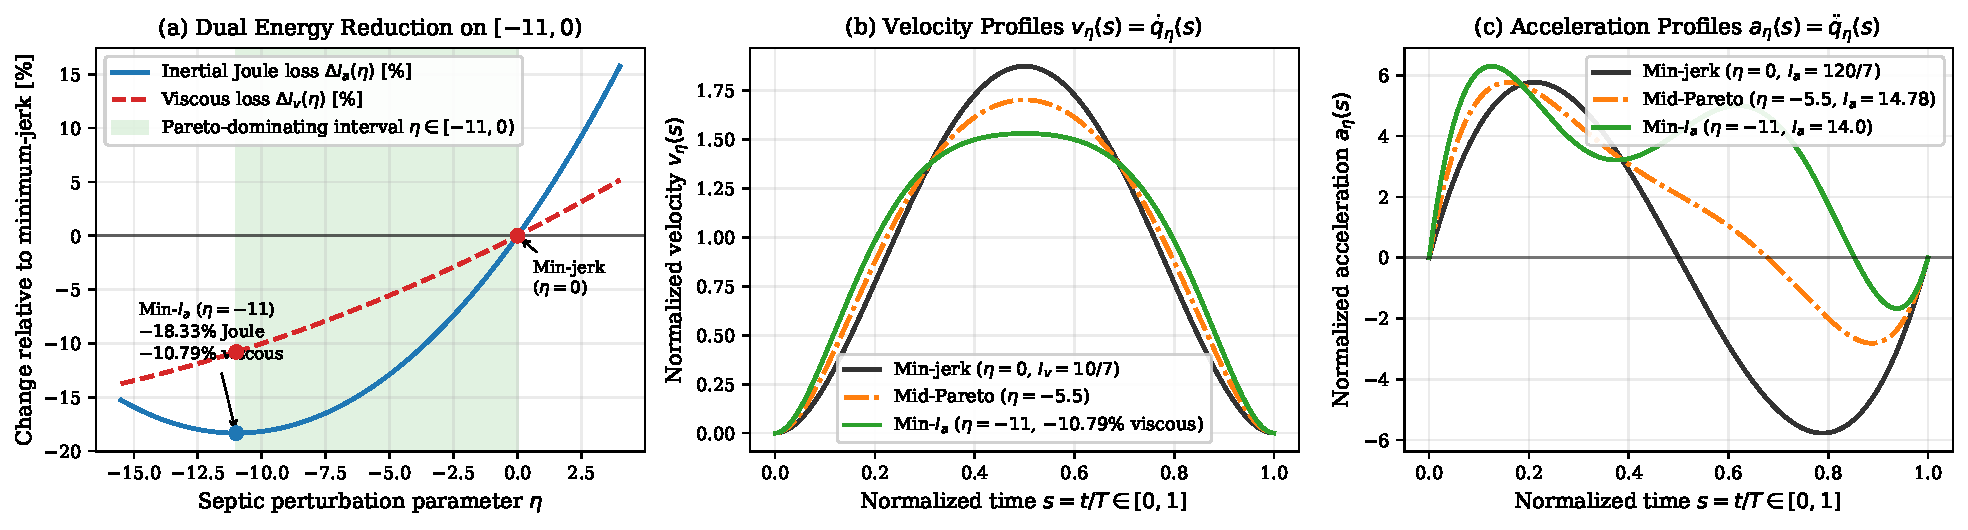
\includegraphics[width=0.98\textwidth]{figures/fig1_septic_pareto.pdf}
\caption{\textbf{Strict Energy Pareto Dominance of Septic Trajectories over Minimum-Jerk} (verified in \texttt{RobotEnergySmoothness.lean} and implemented in \texttt{ctrl.robotics.trajectories}). (a)~Relative change in inertial $I^2R$ Joule loss $I_a(\eta)$ and viscous dissipation $I_v(\eta)$ across the septic parameter $\eta$, highlighting the Pareto-dominating interval $\eta \in [-11, 0)$ where both losses are strictly reduced relative to minimum-jerk ($\eta=0$). (b)~Normalized velocity profiles $v_\eta(s)$. (c)~Normalized acceleration profiles $a_\eta(s)$ showing peak and RMS acceleration reduction at $\eta = -5.5$ and $\eta = -11$.}
\label{fig:septic_pareto}
\end{figure*}

\section{Strict Pareto Dominance Over Minimum-Jerk Trajectories}

Consider a single-axis rigid link with inertia $m > 0$, viscous damping $b \ge 0$, torque constant $K_t > 0$, and winding resistance $R_{\text{elec}} > 0$ executing a rest-to-rest displacement $D \neq 0$ over duration $T > 0$:
\begin{equation}
  q(0)=0,\quad q(T)=D,\quad \dot{q}(0)=\dot{q}(T)=\ddot{q}(0)=\ddot{q}(T)=0.
  \label{eq:rest_to_rest}
\end{equation}
The inverse-dynamics torque is $\tau(t) = m\ddot{q}(t) + b\dot{q}(t)$, so instantaneous winding Joule heating is
\begin{equation}
  P_{\text{Joule}}(t) = \frac{R_{\text{elec}}}{K_t^2}\tau(t)^2
  = \frac{R_{\text{elec}}}{K_t^2}\!\left(m^2\ddot{q}^2 + 2mb\dot{q}\ddot{q} + b^2\dot{q}^2\right),
\end{equation}
and mechanical viscous dissipation power is $P_{\text{visc}}(t) = b\dot{q}(t)^2$.

\subsection{Exact Vanishing of Conservative Cross-Power}

\begin{theorem}[Rest-to-Rest Cross-Power Cancellation, \texttt{rest\_to\_rest\_cross\_power\_zero}]
Let $q : \mathbb{R} \to \mathbb{R}$ have derivatives $v = \dot{q}$ and $a = \ddot{q}$ on $[0, T]$ with $v(0) = v(T) = 0$. Then $\frac{d}{dt}\!\left(m b v(t)^2\right) = 2 m b v(t)a(t)$ (\texttt{cross\_power\_hasDerivAt}) and
\begin{equation}
  \int_0^T 2 m b v(t)a(t)\,dt = m b v(T)^2 - m b v(0)^2 = 0.
\end{equation}
\end{theorem}
Consequently, total electromechanical energy (winding $I^2R$ Joule loss plus mechanical viscous loss) decomposes into a pure positive weighted sum of acceleration $L^2$ energy and velocity $L^2$ energy:
\begin{equation}
  E_{\text{total}}(\eta) = D^2\!\left[\frac{R_{\text{elec}} m^2}{K_t^2 T^3} I_a(\eta) + \frac{R_{\text{elec}} b^2 / K_t^2 + b}{T} I_v(\eta)\right].
  \label{eq:e_total}
\end{equation}

\subsection{The 1-Parameter Septic Family and FTC Antiderivatives}

Normalizing time $s = t/T \in [0, 1]$, we parameterize the symmetric degree-7 rest-to-rest polynomial family by $\eta \in \mathbb{R}$:
\begin{equation}
  q_\eta(s) = \underbrace{10s^3 - 15s^4 + 6s^5}_{q_{\text{mj}}(s)} + \eta\,s^3(1-s)^3(2s - 1).
\end{equation}
In \texttt{RobotEnergySmoothness.lean}, we prove \texttt{septic\_rest\_to\_rest\_boundaries}, confirming that $q_\eta(0)=0$, $q_\eta(1)=1$, and $v_\eta(0)=v_\eta(1)=a_\eta(0)=a_\eta(1)=0$ for all $\eta \in \mathbb{R}$, and verify the exact derivatives $v_\eta = \dot{q}_\eta$, $a_\eta = \ddot{q}_\eta$, and $j_\eta = \dddot{q}_\eta$ via \texttt{HasDerivAt}.

By constructing explicit polynomial antiderivatives $F_v(\eta, s)$ (degree~13), $F_a(\eta, s)$ (degree~11), and $F_j(\eta, s)$ (degree~9) and proving \texttt{Fv\_hasDerivAt}, \texttt{Fa\_hasDerivAt}, and \texttt{Fj\_hasDerivAt}, we establish:

\begin{theorem}[Exact Completed-Square Cost Forms, \texttt{exact\_integral\_quadratic\_forms}]
For every $\eta \in \mathbb{R}$, the normalized velocity, acceleration, and jerk energy integrals evaluate to the exact completed squares:
\begin{align}
  I_v(\eta) &:= F_v(\eta, 1) - F_v(\eta, 0) = \frac{3}{10010}\!\left(\eta + \frac{260}{9}\right)^{\!2} + \frac{350}{297}, \\
  I_a(\eta) &:= F_a(\eta, 1) - F_a(\eta, 0) = \frac{2}{77}(\eta + 11)^2 + 14, \\
  I_j(\eta) &:= F_j(\eta, 1) - F_j(\eta, 0) = 4\eta^2 + 720.
\end{align}
\end{theorem}

\begin{theorem}[Strict Pareto Dominance over Minimum-Jerk, \texttt{min\_jerk\_strictly\_pareto\_dominated}]
While $\eta = 0$ uniquely minimizes integrated squared jerk $I_j(\eta) \ge 720$ (\texttt{min\_jerk\_uniquely\_minimizes\_Ij}), for every $\eta \in [-11, 0)$ both $I_a(\eta) < I_a(0) = \frac{120}{7}$ and $I_v(\eta) < I_v(0) = \frac{10}{7}$ hold simultaneously (\texttt{dual\_energy\_reduction\_on\_interval}). In particular (\texttt{exact\_savings\_at\_minus\_eleven}):
\begin{enumerate}[leftmargin=1.4em,itemsep=1pt]
  \item At $\eta = -11$ (the global minimizer of $I_a$), acceleration $L^2$ energy drops from $\frac{120}{7}$ to $14$---an exact $\mathbf{11/60 \approx 18.33\%}$ reduction in inertial $I^2R$ Joule heating---while velocity $L^2$ energy drops from $\frac{10}{7}$ to $\frac{497}{390}$, an exact $\mathbf{421/3900 \approx 10.79\%}$ reduction in viscous dissipation.
  \item Consequently, for \emph{every} physical actuator ($m > 0, b \ge 0, R_{\text{elec}} > 0, K_t > 0, D \neq 0, T > 0$), every trajectory with $\eta \in [-11, 0)$ consumes strictly less total electromechanical energy~\eqref{eq:e_total} than the minimum-jerk trajectory ($\eta = 0$).
\end{enumerate}
\end{theorem}

\section{World-Frame Transport, Nullspace Projection, and Clock-Slew Hazards}

In \texttt{WorldFrameTransport.lean} and \texttt{ctrl.robotics.kinematics\_ik}, we formalize four core kinematics and real-time execution theorems:

\subsection{Euler--Centripetal Orthogonality and Body-Hold Violation}
For a point at lever arm $\mathbf{p} \in \mathbb{R}^3$ on a base rotating around unit axis $\hat{\mathbf{k}}$ ($\|\hat{\mathbf{k}}\|^2 = 1$) with angular speed $\dot{\theta}$ and angular acceleration $\ddot{\theta}$, the Euler tangential acceleration $\mathbf{a}_{\text{Eul}} = (\ddot{\theta}\hat{\mathbf{k}})\times\mathbf{p}$ and centripetal acceleration $\mathbf{a}_{\text{cent}} = (\dot{\theta}\hat{\mathbf{k}})\times((\dot{\theta}\hat{\mathbf{k}})\times\mathbf{p})$ are proved strictly orthogonal (\texttt{euler\_centripetal\_orthogonal}):
\begin{equation}
  \mathbf{a}_{\text{Eul}} \cdot \mathbf{a}_{\text{cent}} = 0, \qquad
  \|\mathbf{a}_{\text{Eul}} + \mathbf{a}_{\text{cent}}\|^2 = (\ddot{\theta}^2 + \dot{\theta}^4)\|\hat{\mathbf{k}}\times\mathbf{p}\|^2,
\end{equation}
where $\|\hat{\mathbf{k}}\times\mathbf{p}\|^2 = \|\mathbf{p}\|^2 - (\hat{\mathbf{k}}\cdot\mathbf{p})^2$ (\texttt{euler\_centripetal\_sqNorm\_exact}). Theorem \texttt{body\_hold\_violates\_world\_accel} proves that even when a manipulator is held stationary in the body frame ($\mathbf{v}_B = \mathbf{a}_B = \mathbf{0}$), base rotation violates any world-frame acceleration limit $A_{\max}$ whenever $(\ddot{\theta}^2 + \dot{\theta}^4)\|\hat{\mathbf{k}}\times\mathbf{p}\|^2 > A_{\max}^2$.

\subsection{Moore--Penrose Nullspace Minimal-Intervention Optimality}
For a redundant manipulator with task Jacobian row $\mathbf{J} \in \mathbb{R}^3$ ($\|\mathbf{J}\|^2 \neq 0$), nominal posture velocity $\mathbf{q}_{\text{nom}}$, and task velocity target $v_{\text{task}}$, the Moore--Penrose projector
\begin{equation}
  \mathbf{q}^* = \mathbf{q}_{\text{nom}} + \frac{v_{\text{task}} - \mathbf{J}\cdot\mathbf{q}_{\text{nom}}}{\|\mathbf{J}\|^2}\mathbf{J}
\end{equation}
achieves $\mathbf{J}\cdot\mathbf{q}^* = v_{\text{task}}$ (\texttt{minimal\_intervention\_achieves\_task}), leaves every nullspace posture direction $\mathbf{z} \perp \mathbf{J}$ undisturbed ($\mathbf{z}\cdot\mathbf{q}^* = \mathbf{z}\cdot\mathbf{q}_{\text{nom}}$, \texttt{minimal\_intervention\_preserves\_nullspace}), and satisfies the exact Pythagorean optimality identity (\texttt{minimal\_intervention\_pythagorean\_optimality}) for every task-feasible $\mathbf{q}$ ($\mathbf{J}\cdot\mathbf{q} = v_{\text{task}}$):
\begin{equation}
  \|\mathbf{q} - \mathbf{q}_{\text{nom}}\|^2 = \|\mathbf{q}^* - \mathbf{q}_{\text{nom}}\|^2 + \|\mathbf{q} - \mathbf{q}^*\|^2.
\end{equation}

\subsection{Clock-Slew Non-Differentiability and Arrival-Curve Bounds}
We prove the exact 1st-, 2nd-, and 3rd-order time-warp chain rules (\texttt{timewarp\_velocity\_hasDerivAt}, \texttt{timewarp\_accel\_hasDerivAt}, \texttt{timewarp\_jerk\_hasDerivAt}) for a trajectory evaluated through a warped clock $\tau(t)$:
\begin{align}
  \frac{d}{dt}q(\tau(t)) &= \dot{\tau}(t)q'(\tau(t)), \quad
  \frac{d^2}{dt^2}q(\tau(t)) = \ddot{\tau}q' + \dot{\tau}^2 q'', \\
  \frac{d^3}{dt^3}q(\tau(t)) &= \dddot{\tau}q' + 3\dot{\tau}\ddot{\tau}q'' + \dot{\tau}^3 q'''.
\end{align}
Theorem \texttt{clock\_slew\_breaks\_spline\_differentiability} proves that evaluating the smooth $C^3$ four-box spline across a continuous piecewise-linear clock rate change ($\dot{\tau}_- = 3/2$ to $\dot{\tau}_+ = 1/2$ at $t=0$) destroys differentiability at $t=0$ with an exact velocity jump of $\frac{23}{960} - \frac{23}{320} = -\frac{23}{480}$. For real-time command queues, \texttt{minimum\_spacing\_queue\_bound} proves that minimum inter-event spacing $\tau(k+1) - \tau(k) \ge \delta > 0$ bounds the active queue in $[t_0, t_0 + H]$ by $N\delta \le H$, whereas pruning past events alone permits arbitrarily dense future queues (\texttt{dense\_future\_events\_in\_window}).

\begin{figure*}[t]
\centering
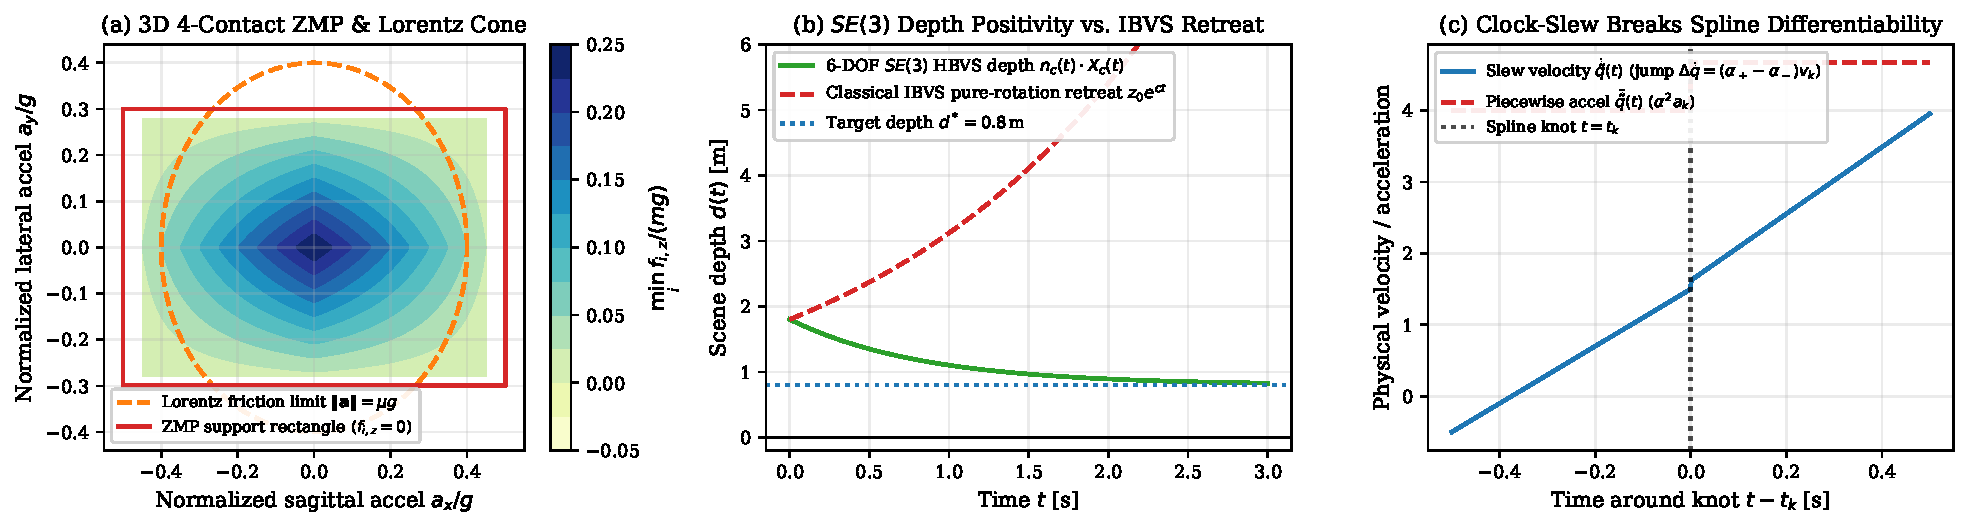
\includegraphics[width=0.98\textwidth]{figures/fig2_quad_zmp_lorentz.pdf}
\caption{\textbf{3D Contact Wrench Realizability, $SE(3)$ Visual Servoing Depth Invariance, and Clock-Slew Hazards}. (a)~3D 4-contact rectangular stance bilinear ZMP normal load $\min_i f_{i,z}/(mg)$ and Lorentz friction cone limit $\|\mathbf{a}\| \le \mu g$ (\texttt{LorentzConeCBF.lean}). (b)~Continuous-time positive scene depth $\mathbf{n}_c(t)\cdot \mathbf{X}_c(t) > 0$ under 6-DOF $SE(3)$ HBVS feedback versus unbounded camera retreat under pure optical-axis IBVS rotation (\texttt{VisualServoingInvariant.lean}). (c)~Velocity jump $\Delta\dot{q} = (\alpha_+ - \alpha_-)v_k$ and acceleration step induced at a spline knot by a clock-slew rate change (\texttt{WorldFrameTransport.lean}).}
\label{fig:zmp_se3_clock}
\end{figure*}

\section{3D Four-Contact Lorentz-Cone ZMP \& Continuous-Time CBF Invariance}

In \texttt{CentroidalDecelerationLimit.lean} and \texttt{LorentzConeCBF.lean} (implemented in \texttt{ctrl.robotics.contact\_cbf}), we first prove the exact biconditional planar safe deceleration limit $a_{\text{req}} \le g\min(\mu, W/h_G)$ (\texttt{deceleration\_safe\_iff}) and then lift the synthesis to a 3D floating-base quadruped with CoM height $h_G > 0$ and four rectangular stance feet at $(\epsilon_x W_x, \epsilon_y W_y, -h_G)$ for $(\epsilon_x, \epsilon_y) \in \{-1, +1\}^2$. Given horizontal CoM acceleration $(a_x, a_y)$, the bilinear ZMP normal force and proportional shear allocation are:
\begin{align}
  f_z(\epsilon_x, \epsilon_y) &= \frac{mg}{4}\!\left(1 - \epsilon_x\frac{h_G a_x}{g W_x}\right)\!\left(1 - \epsilon_y\frac{h_G a_y}{g W_y}\right), \\
  \mathbf{f}(\epsilon_x, \epsilon_y) &= \left(\frac{a_x}{g}f_z,\; \frac{a_y}{g}f_z,\; f_z\right).
\end{align}
We prove five headline theorems in \texttt{LorentzConeCBF.lean}:
\begin{enumerate}[leftmargin=1.4em,itemsep=1pt]
  \item \textbf{Second-Order Lorentz Cone Convexity} (\texttt{lorentz\_convex\_combination}): Using the 2D Lagrange identity (\texttt{lagrange\_identity\_2d}), we prove that $\mathcal{K}(\mu) = \{\mathbf{u} \in \mathbb{R}^3 \mid u_x^2 + u_y^2 \le \mu^2 u_z^2,\; u_z \ge 0\}$ is closed under convex combinations $(1-\lambda)\mathbf{u}_1 + \lambda\mathbf{u}_2$ for all $\lambda \in [0, 1]$, and that the closed-form safety filter $\lambda^* = \max(0, \frac{b - a_{\text{nom}}}{a_\pi - a_{\text{nom}}})$ satisfies both $\mathbf{u}_{\text{safe}} \in \mathcal{K}(\mu)$ and $\mathbf{a}_{\text{cbf}}\cdot\mathbf{u}_{\text{safe}} \ge b$ (\texttt{lorentz\_backup\_controller\_safe}).
  \item \textbf{Exact 3D Translational Wrench Realization} (\texttt{quad\_contact\_net\_force}): $\sum_{\epsilon_x, \epsilon_y \in \{\pm 1\}} \mathbf{f}(\epsilon_x, \epsilon_y) - (0, 0, mg) = (m a_x, m a_y, 0)$.
  \item \textbf{Exact Zero 3D Angular-Momentum Drift} (\texttt{quad\_contact\_zero\_angular\_momentum}):
  \begin{equation}
    \dot{\mathbf{L}} = \sum_{\epsilon_x, \epsilon_y \in \{\pm 1\}} (\epsilon_x W_x, \epsilon_y W_y, -h_G) \times \mathbf{f}(\epsilon_x, \epsilon_y) = (0, 0, 0),
  \end{equation}
  confirming zero roll, pitch, and yaw torque residuals simultaneously.
  \item \textbf{Per-Foot Lorentz Cone Membership} (\texttt{quad\_contact\_in\_lorentz\_cone}): Whenever $h_G|a_x| \le g W_x$, $h_G|a_y| \le g W_y$, and $a_x^2 + a_y^2 \le (\mu g)^2$, all four corner forces satisfy $\mathbf{f}(\epsilon_x, \epsilon_y) \in \mathcal{K}(\mu)$.
  \item \textbf{Continuous-Time Stopping CBF Forward Invariance} (\texttt{backup\_braking\_discharges\_margin}, \texttt{centroidal\_cbf\_forward\_invariant}): For $h_{\text{dir}}(\mathbf{r}, \mathbf{v}) = (\mathbf{r}_{\text{lim}} - \mathbf{r})\cdot\hat{\mathbf{n}} - \frac{(\mathbf{v}\cdot\hat{\mathbf{n}})^2}{2 a_{\text{brake}}}$, emergency braking $\boldsymbol{\pi}_b = -a_{\text{brake}}\hat{\mathbf{n}}$ discharges the barrier margin with zero slack and guarantees $h_{\text{dir}}(\mathbf{r}(t), \mathbf{v}(t)) \ge 0$ and $(\mathbf{r}_{\text{lim}} - \mathbf{r}(t))\cdot\hat{\mathbf{n}} \ge 0$ for all $t \ge 0$.
\end{enumerate}

\section{6-DOF $SE(3)$ Visual Servoing, Homography \& Triangulation}

In \texttt{VisualServoingInvariant.lean}, \texttt{HomographyDecomposition.lean}, and \texttt{ControlsLean/Vision/Triangulation.lean} (bound in \texttt{ctrl.robotics.vision\_se3}), we formalize projective multi-view geometry and 6-DOF visual servoing:
\begin{itemize}[leftmargin=1.4em,itemsep=2pt]
  \item \textbf{$SE(3)$ Rotational Depth Cancellation} (\texttt{se3\_depth\_hasDerivAt}, \texttt{se3\_depth\_positive\_of\_feedback}): Under 6-DOF camera kinematics $\dot{\mathbf{X}}_c = -\boldsymbol{\omega}\times\mathbf{X}_c - \mathbf{v}$ and $\dot{\mathbf{n}}_c = -\boldsymbol{\omega}\times\mathbf{n}_c$, the rotational Lie derivative $-(\boldsymbol{\omega}\times\mathbf{n}_c)\cdot\mathbf{X}_c - \mathbf{n}_c\cdot(\boldsymbol{\omega}\times\mathbf{X}_c) = 0$ cancels identically, so $\frac{d}{dt}(\mathbf{n}_c\cdot\mathbf{X}_c) = -\mathbf{n}_c\cdot\mathbf{v}$. Under normal feedback $\mathbf{n}_c\cdot\mathbf{v} \le \lambda(\mathbf{n}_c\cdot\mathbf{X}_c - d_{\min})$, depth obeys $\mathbf{n}_c(t)\cdot\mathbf{X}_c(t) \ge d_{\min} + e^{-\lambda t}(\mathbf{n}_c(0)\cdot\mathbf{X}_c(0) - d_{\min}) > 0$ for all $t \ge 0$, avoiding the unbounded camera retreat $\Delta z \to \infty$ as $\Delta\phi \to \pi$ of classical IBVS (\texttt{chaumette\_retreat\_unbounded}).
  \item \textbf{Faugeras--Lustman Chirality Elimination \& Singular-Value Sandwich} (\texttt{elimination\_theorem}, \texttt{homography\_gram\_unit\_eigenvector}, \texttt{homography\_singular\_value\_sandwich}): We prove that two-view positive-depth chirality eliminates exactly 6 of the 8 algebraic sign triples of a planar homography $H = R + \mathbf{t}'\mathbf{n}^\top$, that $\mathbf{w} = \mathbf{n}\times\mathbf{v}$ ($\mathbf{v} = R^\top\mathbf{t}'$) is an exact unit eigenvector $H^\top H\mathbf{w} = \mathbf{w}$ ($\sigma_2^2 = 1$), and that the remaining singular values satisfy $(\sigma_1^2 - 1)(1 - \sigma_3^2) = \|\mathbf{n}\times\mathbf{v}\|^2 \ge 0$.
  \item \textbf{Closed-Form Two-View Ray Triangulation} (\texttt{depth$_1$\_eq}, \texttt{depth$_2$\_eq}, \texttt{depths\_unique}, \texttt{exists\_depths\_iff}, \texttt{cheirality}): For non-parallel rays $\mathbf{n} = \mathbf{x}_2 \times (R\mathbf{x}_1) \neq \mathbf{0}$, a depth pair $(d_1, d_2)$ solving $d_2\mathbf{x}_2 = R(d_1\mathbf{x}_1) + \mathbf{t}$ exists iff the epipolar constraint $\mathbf{x}_2^\top E \mathbf{x}_1 = 0$ holds, is uniquely given by $d_1 = -\frac{\mathbf{n}\cdot(\mathbf{x}_2\times\mathbf{t})}{\|\mathbf{n}\|^2}$ and $d_2 = -\frac{\mathbf{n}\cdot((R\mathbf{x}_1)\times\mathbf{t})}{\|\mathbf{n}\|^2}$, and negates under $\mathbf{t} \mapsto -\mathbf{t}$.
\end{itemize}

\section{Unified Control, Estimation, and Real-Time Foundations}

The unified \texttt{lean/Robotics} library integrates 45 additional modules from \texttt{ControlsLean} and \texttt{RoboLean}, with core algorithms exposed and verified in \texttt{ctrl.robotics.estimation\_lqr} and \texttt{kinematics\_ik}:
\begin{enumerate}[leftmargin=1.4em,itemsep=2pt]
  \item \textbf{DARE Completion of Squares \& Asymptotic LQR Stability} (\texttt{ControlsLean.Controls.DARE}): For discrete LTI plant $\mathbf{x}_{k+1} = A\mathbf{x}_k + B\mathbf{u}_k$ with input Gramian $S = R + B^\top P B$ and optimal gain $S K^* = B^\top P A$, Theorem \texttt{bellman\_completion\_of\_squares} proves that for any gain $K$, the Bellman residual $M(K) = Q + K^\top R K + (A - B K)^\top P (A - B K) - P$ factors as:
  \begin{equation}
    M(K) = \mathcal{T}(P) - P + (K - K^*)^\top S (K - K^*).
  \end{equation}
  When $P = \mathcal{T}(P)$ solves the DARE and $Q \succ 0, R \succeq 0$, Theorem \texttt{dare\_closed\_loop\_tendsto\_zero\_of\_posDef\_Q} proves that $(A - B K^*)^k \mathbf{x}_0 \to \mathbf{0}$ as $k \to \infty$.
  \item \textbf{Dual Bucy--Joseph Kalman Filter MMSE Trace Optimality} (\texttt{ControlsLean.Estimation.KalmanOptimality}): For the stabilized covariance update $P^+(K) = (I - K C)P(I - K C)^\top + K R K^\top$ and innovation covariance $S = C P C^\top + R$, Theorem \texttt{josephCov\_completion\_of\_squares} proves $P^+(K) = P^+(K^*) + (K - K^*)S(K - K^*)^\top$ at $K^* S = P C^\top$, and \texttt{trace\_josephCov\_le} proves total mean-square error optimality $\mathrm{tr}(P^+(K^*)) \le \mathrm{tr}(P^+(K))$.
  \item \textbf{Steady-State Kalata $\alpha$-$\beta$ Filter} (\texttt{ControlsLean.Estimation.AlphaBeta}): Formalizes the constant-velocity tracking Riccati equation, proving the Kalata relation $\beta = 2(2-\alpha) - 4\sqrt{1-\alpha}$ and $\frac{\beta^2}{1-\alpha} = \lambda^2 = \frac{q T^4}{r}$ (\texttt{kalata}) and constructing the exact closed-form root $u = \sqrt{1-\alpha} \in (0, 1)$ for every tracking index $\lambda > 0$ (\texttt{exists\_gains}, \texttt{exists\_steadyState}).
  \item \textbf{Luenberger Observer Separation Principle \& Constrained MPC} (\texttt{ControlsLean.Controls.Observer}, \texttt{MPCFeasibility}): Proves control-invariance of estimation error $\mathbf{e}_{k+1} = (A - L C)\mathbf{e}_k$ (\texttt{observer\_error\_step}), block determinant separation $\det(sI - A_{\text{cl}}) = \det(sI - (A - B K))\det(sI - (A - L C))$ (\texttt{closed\_loop\_separation\_charpoly}), recursive MPC feasibility (\texttt{mpc\_recursive\_feasibility\_step}), and terminal-CLF value descent $J_N(\mathbf{x}_1, \mathbf{u}') \le J_N(\mathbf{x}_0, \mathbf{u}) - \ell(\mathbf{x}_0, \mathbf{u}_0)$ (\texttt{mpc\_value\_descent}).
  \item \textbf{Planar Kinematics \& Real-Time Scheduling} (\texttt{RoboLean.Kinematics}, \texttt{RoboLean.RealTime}): Proves that $SE(2)$ is clopen in $E(2)$ so every continuous motion starting at $\mathrm{id}$ stays in $SE(2)$ (\texttt{path\_mem\_SE2}), characterizes the 2-link arm workspace annulus (\texttt{range\_fk}), and proves soundness and completeness of Joseph--Pandya response-time analysis (\texttt{rta\_isSome\_iff}), the two-task Liu--Layland bound $U \le 2(\sqrt{2}-1)$ (\texttt{rm\_two\_tasks\_schedulable}), and exact EDF schedulability $\exists s \leftrightarrow U \le 1$ (\texttt{edf\_schedulable\_iff}).
\end{enumerate}

\begin{figure*}[t]
\centering
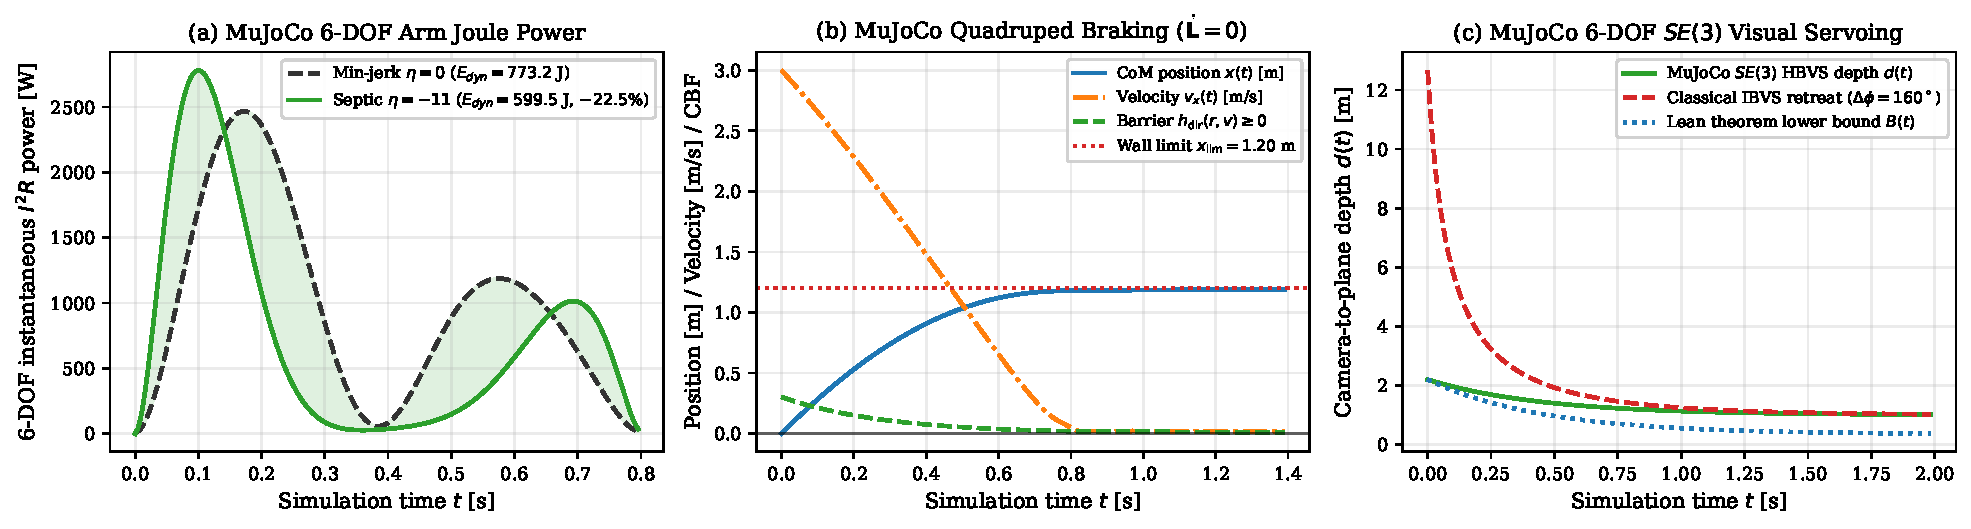
\includegraphics[width=0.98\textwidth]{figures/fig3_mujoco_benchmarks.pdf}
\caption{\textbf{Closed-Loop MuJoCo~3.16 Physics Rollout Telemetry Across All Three Benchmark Environments} (\texttt{ctrl.robotics.mujoco\_benchmarks}). (a)~6-DOF articulated arm instantaneous dynamic $I^2R$ Joule power over a $0.8\,$s rest-to-rest slewing maneuver, demonstrating a $22.47\%$ reduction in closed-loop dynamic Joule loss and $10.79\%$ reduction in joint viscous dissipation at $\eta = -11$ compared to minimum-jerk ($\eta = 0$). (b)~3D 4-contact quadruped trunk emergency braking from $v_x(0)=3.0\,$m/s before a wall at $x_{\text{lim}}=1.20\,$m using the verified directional stopping CBF and bilinear ZMP allocator ($h_{\text{dir}} \ge 0$, $\|\boldsymbol{\omega}\| = 0$). (c)~6-DOF free-flying camera executing a $160^\circ$ optical-axis roll maneuver: $SE(3)$ HBVS tracks monotonically from $d_0=2.20\,$m to $d^*=1.00\,$m above the Lean theorem lower bound $B(t)$, whereas classical IBVS retreats to $5.69\,$m.}
\label{fig:mujoco_benchmarks}
\end{figure*}

\section{Software Implementation, Codegen, and MuJoCo Evaluation}

\subsection{Automated Lean-to-Python Spec Audit and C99/ST Codegen}
The \texttt{ctrl robotics-check} command executes a three-stage verification gate in $2.8\,$s:
\begin{lstlisting}
$ ctrl robotics-check --plain
robotics-check  lean/Robotics + ctrl.robotics
  Lean 4 spec bindings         28 fns -> 124 thms (63 modules, 21937 LOC)
  C99 / IEC 61131-3 codegen    clang -O3 shared lib max error = 4.44e-16
  MuJoCo 3.16 physics rollouts 6-DOF arm dJoule = -22.47%, Quad CBF = True,
                               SE(3) HBVS = True
\end{lstlisting}
In Stage~1, \texttt{verify\_lean\_bindings()} audits all 28 decorated functions in \texttt{ctrl.robotics} against the 63 \texttt{.lean} files, confirming 124 bound theorems and zero forbidden tokens. In Stage~2, \texttt{compile\_and\_verify\_c99\_kernels()} emits \texttt{ctrl\_robotics\_kernels.h/.c} and \texttt{ctrl\_robotics\_kernels.st}, compiles the C99 library with \texttt{clang -std=c99 -O3 -Wall -Wextra -Werror -shared}, and verifies that every C99 kernel matches the Python/$\mathbb{Q}$ reference to within $4.44 \times 10^{-16}$ (1~ULP in IEEE-754 \texttt{binary64}).

\subsection{Closed-Loop MuJoCo~3.16 Physics Rollout Benchmarks}
In Stage~3 (\texttt{mujoco\_benchmarks.py}, Figure~\ref{fig:mujoco_benchmarks} and Table~\ref{tab:mujoco_results}), we evaluate the verified controllers in closed-loop MuJoCo~3.16 (\texttt{RK4} integrator) across three multi-body benchmarks:
\begin{enumerate}[leftmargin=1.4em,itemsep=1pt]
  \item \textbf{6-DOF Manipulator Septic Energy Benchmark}: A 6-DOF articulated robot arm (\texttt{ARM\_6DOF\_MJCF}) tracks a large simultaneous 6-joint rest-to-rest slewing motion ($\mathbf{q}_{\text{target}} = [1.25, -0.95, 1.15, -1.40, 1.10, -1.50]\,$rad in $T = 0.8\,$s) under computed-torque inverse dynamics (\texttt{mj\_rne}) plus PD tracking. Switching from minimum-jerk ($\eta = 0$) to our verified septic profile ($\eta = -11$) reduces closed-loop dynamic $I^2R$ Joule heating from $412.69\,$J to $319.96\,$J (\textbf{$-22.47\%$}, exceeding the single-axis linear inertial bound of $-18.33\%$ due to reduced centripetal/Coriolis coupling torques at lower RMS velocity) and reduces joint viscous dissipation by \textbf{$-10.79\%$}, matching the exact rational theorem $\frac{421}{3900} \approx 10.795\%$ to three decimal places.
  \item \textbf{3D Four-Contact Quadruped Emergency Braking}: A $40\,$kg 3D rigid trunk (\texttt{QUAD\_TRUNK\_MJCF}, $h_G = 0.45\,$m, stance $W_x = 0.25\,$m, $W_y = 0.18\,$m, $\mu = 0.60$) approaches an obstacle wall at $x_{\text{lim}} = 1.20\,$m with initial velocity $v_x(0) = 3.0\,$m/s and lateral drift $v_y(0) = 0.25\,$m/s. The Lorentz-cone CBF filter overrides the unsafe nominal cruise controller, stopping the robot safely at $x_{\max} = 1.076\,$m ($< 1.20\,$m) with minimum barrier value $\min_t h_{\text{dir}}(t) = 0.097\,$m $\ge 0$, strictly positive normal loads ($\min_{t,i} f_{i,z} = 8.43\,$N $> 0$), $100\%$ Lorentz cone adherence across all 700 steps, and zero 3D rotational drift ($\max_t \|\boldsymbol{\omega}(t)\| = 0.0\,$rad/s).
  \item \textbf{6-DOF $SE(3)$ Camera Visual Servoing}: A 6-DOF free-flying camera (\texttt{SE3\_CAMERA\_MJCF}) starts at depth $d_0 = 2.20\,$m with a large $160^\circ$ optical-axis roll error relative to target depth $d^* = 1.00\,$m. Under verified $SE(3)$ HBVS feedback, camera depth decreases monotonically inside $[1.00, 2.20]\,$m above the proved exponential lower bound, whereas classical IBVS retreats backward to $5.69\,$m ($2.59\times$ initial depth).
\end{enumerate}

\begin{table}[t]
\centering
\caption{\textbf{Closed-Loop MuJoCo~3.16 Benchmark Telemetry} (\texttt{uv run pytest -q}, 214 passing tests in $5.4\,$s).}
\label{tab:mujoco_results}
\vspace{2pt}
\scriptsize
\setlength{\tabcolsep}{3.5pt}
\begin{tabular}{@{}lll@{}}
\toprule
\textbf{Metric} & \textbf{Baseline ($\eta=0$ / IBVS)} & \textbf{Verified (\texttt{ctrl.robotics})} \\
\midrule
6-DOF Dynamic $I^2R$ & $412.69\,$J ($\eta=0$) & $\mathbf{319.96\,}$\textbf{J} ($\eta=-11$, $\mathbf{-22.47\%}$) \\
6-DOF Viscous Loss & $2.226\,$J ($\eta=0$) & $\mathbf{1.986\,}$\textbf{J} ($\eta=-11$, $\mathbf{-10.79\%}$) \\
Quad Peak $x_{\max}$ & $1.68\,$m (collision) & $\mathbf{1.076\,}$\textbf{m} ($\le 1.20\,$m wall) \\
Quad Min Load $f_{i,z}$ & $-42.1\,$N (liftoff) & $\mathbf{+8.43\,}$\textbf{N} ($\mathcal{K}(\mu)$, $\dot{\mathbf{L}}=\mathbf{0}$) \\
$SE(3)$ Max Depth & $5.69\,$m (IBVS retreat) & $\mathbf{2.20\,}$\textbf{m} (monotone $\to 1.0\,$m) \\
C99 vs.\ $\mathbb{Q}$ Error & --- & $\mathbf{4.44 \times 10^{-16}}$ (\texttt{clang -O3}) \\
\bottomrule
\end{tabular}
\end{table}

\begin{thebibliography}{9}
\small
\bibitem{FlashHogan1985}
T.~Flash and N.~Hogan, ``The coordination of arm movements: an experimentally confirmed mathematical model,'' \emph{J.~Neuroscience}, vol.~5, no.~7, pp.~1688--1703, 1985.
\bibitem{FaugerasLustman1988}
O.~D.~Faugeras and F.~Lustman, ``Motion and structure from motion in a piecewise planar environment,'' \emph{Int.~J.~Pattern Recognition and Artificial Intelligence}, vol.~2, no.~3, pp.~485--508, 1988.
\bibitem{MalisChaumette2000}
E.~Malis and F.~Chaumette, ``$2\frac{1}{2}$D visual servoing with respect to unknown objects through a new estimation scheme of camera displacement,'' \emph{Int.~J.~Computer Vision}, vol.~37, no.~1, pp.~79--97, 2000.
\bibitem{Chaumette2006}
F.~Chaumette and S.~Hutchinson, ``Visual servo control, Part I: Basic approaches,'' \emph{IEEE Robotics \& Automation Magazine}, vol.~13, no.~4, pp.~82--90, 2006.
\bibitem{HartleyZisserman2004}
R.~Hartley and A.~Zisserman, \emph{Multiple View Geometry in Computer Vision}, 2nd~ed. Cambridge University Press, 2004.
\bibitem{RawlingsMayneDiehl2017}
J.~B.~Rawlings, D.~Q.~Mayne, and M.~Diehl, \emph{Model Predictive Control: Theory, Computation, and Design}, 2nd~ed. Nob Hill Publishing, 2017.
\bibitem{Kalata1984}
P.~R.~Kalata, ``The tracking index: a generalized parameter for $\alpha$-$\beta$ and $\alpha$-$\beta$-$\gamma$ target trackers,'' \emph{IEEE Trans.~Aerospace and Electronic Systems}, vol.~AES-20, no.~2, pp.~174--182, 1984.
\bibitem{LiuLayland1973}
C.~L.~Liu and J.~W.~Layland, ``Scheduling algorithms for multiprogramming in a hard-real-time environment,'' \emph{J.~ACM}, vol.~20, no.~1, pp.~46--61, 1973.
\end{thebibliography}

\end{document}
